\documentclass[A4paper,12pt]{article}
% \setlength{\headheight}{14.49998pt}

% Packages
\usepackage[margin=1in]{geometry}
\usepackage{setspace}
\usepackage{titlesec}
\usepackage{booktabs}
\usepackage{array}
\usepackage{longtable}
\usepackage{hyperref}
\usepackage{parskip}
\usepackage{enumitem}
\usepackage{fancyhdr}
\usepackage{graphicx}
\usepackage{fontenc}
\usepackage{inputenc}


% --- Math & fonts ---
\usepackage[centertags]{amsmath}
\usepackage{amsfonts}
\usepackage{amssymb}
\usepackage{amsthm}
\usepackage{latexsym}
\usepackage{mathptmx}

% --- Graphics & figures ---
\usepackage{graphicx}
\usepackage{epsfig}
\usepackage{epstopdf}
\usepackage{float}
\usepackage{placeins}
\usepackage{caption}
\usepackage{adjustbox}
\usepackage{rotating}
\usepackage{lscape}

% --- Colors, frames & boxes ---
\usepackage[table,xcdraw]{xcolor}
\usepackage{framed}
\usepackage{fancybox}
\usepackage{color}

% --- Tables ---
\usepackage{booktabs}
\usepackage{threeparttable}

% --- Formatting ---
\usepackage{newlfont}
\usepackage{setspace}
\usepackage{kantlipsum}
\usepackage{fancyhdr}
\usepackage[normalem]{ulem}
\useunder{\uline}{\ul}{}

% Section formatting
\titleformat{\section}{\large\bfseries}{\thesection}{1em}{}
\titleformat{\subsection}{\normalsize\bfseries}{\thesubsection}{1em}{}

\hypersetup{
    colorlinks=true,
    linkcolor=black,
    urlcolor=blue,
    citecolor=black
}

\begin{document}

% -----------------------------------------------
% Title Page
% -----------------------------------------------
\begin{center}

\textsc{\huge COMSATS University Islamabad \\[0.6cm]   Attock Campus}\\[0.6cm]


\includegraphics[height=3.5cm]{comsats.jpg}

\vspace{0.8cm}

{\LARGE \textbf{Project Proposal}}\\[0.8cm]

for\\[0.8cm]
{\Large\textbf{Jawhar}}\\[0.4cm]

{\LARGE AI Powered Classical Arabic and Quran Understanding Platform}\\[0.8cm]

by\\[0.4cm]

Meher Ali \\[0.2cm]
Hammad Ali  \\[0.8cm]

CIIT/FA23-BCS-059/ATK \\[0.2cm]
CIIT/FA23-BCS-007/ATK \\[1.2cm]

\textbf{Supervisor}\\[0.4cm]
Mr. Babar Shahzad\\[2.7cm]

\textbf{Bachelor of Science in Computer Science (2023--2027)}

\end{center}

% -----------------------------------------------
% Supervisor Approval Page
% -----------------------------------------------
\newpage
\begin{center}

\LARGE{AI Powered Arabic Learning and Quran Understanding Platform}\\
\vspace{0.5in}

\normalsize{By}\\
\vspace{0.5in}
\large{\textit{Hammad Ali}\\
{\textit{CIIT/FA23-BCS-007/ATK}}}\\
\large{\textit{Meher Ali}\\
{\textit{CIIT/FA23-BCS-059/ATK}}}\\
\vspace{0.5in}

\normalsize{As the supervisor, I have reviewed the proposed project and found it to be feasible, relevant, and aligned with academic and industry standards. I recommend this project for evaluation by the committee to assess its viability and grant approval for further development.}\\
\end{center}

\vspace{0.1in}

Supervisor Signature:\line(1,0){280}
\begin{center}
\normalsize{Mr. Babar Shahzad\\
Department of Computer Science, (CUI) Attock Campus}
\end{center}
\vspace{0.1in}

% -----------------------------------------------
% Project Summary
% -----------------------------------------------
\newpage
\section*{Project Summary}
\addcontentsline{toc}{section}{Project Summary}

Understanding the Quran in its original Classical Arabic is a shared goal for over 1.8 billion Muslims around the world. Most of them are not native Arabic speakers, and very few have access to effective self-paced tools for learning Arabic grammar. Platforms that do exist either focus only on vocabulary, depend on paid tutors, or are built for academic researchers rather than everyday learners.

The core difficulty lies in two fundamental disciplines: Sarf (morphology, i.e.\ the study of word roots and patterns) and Nahw (syntax, i.e.\ the rules governing sentence structure). These topics are largely absent from modern language learning apps. As a result, learners may recognise individual words but still struggle to understand complete sentence meanings or grammatical structure.

This project proposes \textbf{Jawhar}, an AI-powered, cross-platform learning system for Classical Arabic and Quranic comprehension. The system brings together a Sarf engine built on CAMeL Tools, a Nahw parser powered by Farasa NLP, a conversational AI tutor using Gemini 3.1 Flash-Lite, a vocabulary spaced repetition system based on the SM-2 algorithm, and an adaptive personalized learning path.

The primary dataset is the Quranic Arabic Corpus, which contains detailed linguistic annotations for all 77,430 words of the Quran.

This platform targets a clear and unaddressed gap. It brings rigorous linguistic analysis into a clean, mobile-first learning experience. The aim is to make Classical Arabic grammar genuinely accessible to learners at all levels, particularly in regions like Pakistan where motivation is high but resources are limited.

% -----------------------------------------------
% Table of Contents
% -----------------------------------------------
%\newpage
%\tableofcontents
\newpage

% -----------------------------------------------
% Section 1: Introduction
% -----------------------------------------------
\section{Introduction}

Language has always been humanity's most consequential barrier and its most powerful bridge. For most of recorded history, learning a language outside one's native environment meant physical proximity to speakers, years of immersive exposure, or access to formal institutions, conditions unavailable to the vast majority of the world's population. The twentieth century began to dismantle these barriers incrementally. Cassette tapes brought foreign speech into households that had never hosted a native speaker. CD-ROM software and early internet resources made dictionaries, grammars, and reading materials globally available. The smartphone era then accelerated access at a scale previously unimaginable: interactive apps, spaced repetition systems, and AI-driven tutors collectively brought language learning to hundreds of millions of ordinary people with nothing more than a phone and motivation. Yet even as these tools matured, they remained concentrated around a narrow set of high-resource languages.
% Languages whose learning is inseparable from a deep textual and scholarly tradition, and whose grammar is a prerequisite for accessing centuries of written heritage, were largely left behind. The infrastructure of modern language technology was built for the learner of French or Mandarin, not for the learner whose goal is to comprehend a classical text in its original form.

Arabic is the fifth most widely spoken language in the world and the liturgical language of Islam.
Classical Arabic, as preserved in the Quran, holds a unique place: it is the direct medium of Quranic
revelation and the foundation of over 1,400 years of Islamic scholarship. For approximately 1.8 billion
Muslims worldwide, the vast majority of whom are not native Arabic speakers, understanding the Quran
in its original language is both a religious aspiration and a real educational challenge.

The Quran's linguistic precision rests on two interconnected disciplines: \textbf{Sarf} (morphology),
which is the science of Arabic word formation, roots, and patterns, and \textbf{Nahw} (syntax), which
governs sentence structure, word roles, and case endings (i'rab). A single change in a word's
morphological pattern or case ending can shift the entire meaning of an ayah. Mastery of both
disciplines is therefore not optional for anyone seeking genuine Quranic comprehension; it is a
prerequisite.

Despite the scale of this need, the digital landscape for Classical Arabic learning remains severely
fragmented. On one end, vocabulary-focused apps such as Quranic App and Kalaam help users
recognise common words but provide no grammar instruction whatsoever. On the other end,
corpus.quran.com offers world-class linguistic annotation for all 77,430 words of the Quran,
complete with morphological tags, part-of-speech labels, and syntactic treebanks. However, it
is a desktop-only research tool designed for graduate linguists, not for the general Muslim
learner. Its creator, Kais Dukes of the University of Leeds, publicly
acknowledged back in 2010 that the corpus needed a simpler, beginner-oriented derivative to
serve everyday learners. That gap has not been filled since.

The proposed platform is a full-stack native mobile application built with Kotlin Multiplatform,
targeting Android as its primary platform with a clean interface. It brings
the same linguistic depth as corpus.quran.com into a beginner-friendly, AI-powered, and gamified
interface. It integrates an NLP-powered Sarf Engine for root analysis and morphological
decomposition, a Nahw Parser for sentence annotation with classical grammatical roles, a Gemini
3.1 Flash-Lite powered AI Tutor grounded in Classical Arabic pedagogy, a Spaced Repetition
vocabulary system, and an adaptive personalized learning path.

The project is relevant to the fields of Natural Language Processing, Educational Technology, and
Human-Computer Interaction, and it contributes a practical, deployable system that can reach
millions of Quran learners worldwide.



\section{Literature Review}

This section explores the academic foundations, computational tools, existing applications, and
empirical research that underpin the proposed platform, identifying the gaps that this work aims
to address.

The foundational computational resource for this project is the Quranic Arabic Corpus, introduced
by Dukes and Habash \cite{dukes2010}, which provides morphological segmentation, part-of-speech
tagging, and syntactic dependency annotations for all 77,430 words of the Quran using the classical
i'rab framework. This work established the gold standard for Quranic linguistic analysis and has
since underpinned the majority of subsequent research in Quranic NLP. Complementing this,
Habash \cite{habash2010} offers a comprehensive treatment of Arabic morphology, syntax, and
computational processing challenges in his book \textit{Introduction to Arabic Natural Language
Processing}, which remains the definitive academic reference for researchers and developers working
with Arabic text. The broader scholarly significance of this domain was highlighted by
Atwell et al.\ \cite{atwell2010}, who framed the problem of ``Understanding the Qur'an'' as a
grand AI challenge requiring advances in reasoning, knowledge representation, and natural language
understanding, positioning Quranic NLP as one of the most meaningful open problems in the field.
A recent systematic review by Bashir et al.\ \cite{bashir2022}, published in \textit{Artificial
Intelligence Review}, surveyed over two decades of Quranic NLP research spanning morphological
analysis, syntactic parsing, semantic search, and recitation correction, and confirmed that while
significant academic progress has been made, the gap between research-grade tools and accessible
learning applications remains wide and largely unaddressed.

On the tooling side, the two NLP engines that form the computational core of this project are
both well-established in the academic literature. Obeid et al.\ \cite{obeid2020} presented
CAMeL Tools, an open-source Python toolkit developed at New York University Abu Dhabi that
provides a state-of-the-art morphological analyser capable of disambiguating Arabic words and
extracting root, pattern, lemma, tense, voice, gender, and number features. Its design targets
Classical and Modern Standard Arabic, making it directly applicable to Quranic text without
any adaptation. Abdelali et al.\ \cite{abdelali2016} introduced Farasa, a fast and accurate
Arabic segmenter, POS tagger, and dependency parser developed at the Qatar Computing Research
Institute (QCRI), reporting near state-of-the-art accuracy across multiple Arabic NLP benchmarks.
Farasa's dependency parser provides the syntactic backbone for the Nahw Parser module, enabling
automated identification of classical grammatical roles such as fa'il, maf'ul, mubtada, and
khabar in Quranic sentences. Together, these two tools represent the most capable open-source
Arabic NLP pipeline available for this kind of pedagogical system, and their integration into a
single consumer-facing application is a contribution in its own right. The challenge of Arabic
syntactic dependency parsing has been further addressed by Taji et al.\ \cite{taji2017}, who
developed a Universal Dependency treebank for Arabic, providing standardised syntactic annotations
that serve as the evaluation framework against which the Nahw Parser module in this project is
benchmarked. A broader linguistic foundation is provided by Farghaly and Shaalan \cite{farghaly2009},
whose comprehensive survey of Arabic NLP challenges and solutions catalogues the unique difficulties
of Arabic morphological richness, diglossia, and orthographic ambiguity that make Quranic Arabic
computationally distinct from both Modern Standard Arabic and dialectal Arabic. Earlier,
Pasha et al.\ \cite{pasha2014} introduced MADAMIRA, a comprehensive morphological analysis and
disambiguation tool, which provides the baseline performance standard against which CAMeL Tools
is compared in evaluations.

The vocabulary retention component of this system draws on the foundational memory research of
Ebbinghaus \cite{ebbinghaus1885}, whose forgetting curve model established that memory decays
exponentially without reinforcement and that strategically timed reviews restore and extend
retention. This theoretical basis was operationalised by Wozniak in the SM-2 algorithm
(SuperMemo, 1990), which dynamically schedules flashcard reviews based on per-item recall
ratings and an ease factor, leading to progressively longer inter-repetition intervals as
retention strengthens. The SM-2 algorithm forms the basis of widely-used learning software
including Anki and Mnemosyne. Settles and Meeder \cite{settles2016} extended this work by
formalising spaced repetition as a machine learning task, presenting a trainable model derived
from large-scale Duolingo learner data that adapts interval scheduling to individual learner
recall patterns. Seibert Hanson and Brown \cite{seibert2020} confirmed through a classroom
study using Anki that mobile-assisted spaced repetition yields measurable retention gains over
conventional study methods, and Kim and Webb \cite{kim2022} strengthened this further with a
meta-analysis of 63 spaced practice studies in second language acquisition, finding a significant
overall effect size and concluding that spaced practice is one of the most robust and replicable
interventions in language learning research. Its application to Quranic vocabulary is particularly
well-suited because root-based word grouping allows the algorithm to reinforce both individual
word recognition and morphological pattern recall simultaneously across review sessions.

From the perspective of existing products, the landscape reveals a consistent pattern of partial
solutions. The Quranic Arabic Corpus (\texttt{corpus.quran.com}) provides unmatched linguistic
depth but is a desktop-only, researcher-facing tool with no learning path, AI integration, or
mobile support \cite{dukes2010}. General-purpose language apps such as Duolingo and Mondly teach
Modern Standard Arabic, which differs structurally from Classical Quranic Arabic in vocabulary,
morphological patterns, and syntactic constructions, and neither includes any Sarf or Nahw
curriculum. Tarteel AI \cite{tarteel2024} focuses exclusively on recitation memorisation through
speech recognition and offers nothing toward grammatical comprehension. Live-tutoring platforms
such as Buruj Academy and Kalimah Center do provide Nahw and Sarf instruction but require paid,
synchronous sessions, making them inaccessible to learners in lower-income regions such as
Pakistan.

Two noteworthy mobile applications from Furqan Apps address parts of this space but fall short
of an integrated solution. The first, \textit{Sarf} \cite{furqan_sarf2026}, is a dedicated
Arabic verb conjugation tool that covers full conjugation tables for all 14 grammatical persons
across trilateral verb forms I through X, both active and passive voices, and all major tenses
including the jussive, subjunctive, and emphatic. It also bundles the complete text of Qatr
al-Nada by Ibn Hisham in four languages and integrates Lane's Arabic-English Lexicon for root
and word lookups. The app operates entirely offline and is polished in design, making it a
capable standalone reference for Sarf study. However, it has no connection to the Quranic
corpus, no Nahw parsing, no adaptive learning path, no AI tutor, and no spaced repetition system.
It is a reference tool, not a learning platform. The second, \textit{Quran} by Furqan Apps
\cite{furqan_quran2026}, is a more comprehensive Quran study application offering high-quality
Uthmani and IndoPak Nastaleeq text, Tajweed colour-coding, word-by-word grammatical analysis
(i'rab) sourced from Al-Karbasi and Muyassar, multiple Arabic and English tafsirs, visual
dependency graphs for syntactic relationships, Lane's Lexicon integration, and audio recitation
with multiple reciters. It is a genuinely content-rich application. However, it is primarily a
reading and reference tool rather than a structured learning platform: it provides no onboarding
assessment, no adaptive curriculum, no spaced repetition vocabulary system, no AI tutor capable
of interactive dialogue, no gamification layer, and no progress tracking. A learner with no
prior Arabic background cannot use it to systematically acquire Sarf and Nahw knowledge.

The AI Tutor module of the proposed platform is supported by empirical research on LLM-based
conversational agents in language education. Zhang and Huang \cite{zhang2024} demonstrated
through a controlled eight-week experiment that second language learners assisted by an LLM-based
chatbot significantly outperformed a control group on both receptive and productive vocabulary
post-tests, providing direct empirical support for the AI Tutor module as a learning intervention
and not merely a convenience feature. The platform's gamification layer, consisting of streaks,
badges, and leaderboards, draws on the foundational definition provided by
Deterding et al.\ \cite{deterding2011} and is supported by the systematic review of
Hamari et al.\ \cite{hamari2014}, who found consistent positive effects on motivation and
engagement across 24 empirical gamification studies.

No existing platform integrates all five dimensions, namely morphological analysis, syntactic
parsing, AI-powered tutoring, spaced repetition vocabulary, and an adaptive learning path, into
a single coherent, self-paced, mobile-first application targeting Quranic Arabic.

\vspace{1em}
\begin{longtable}{|>{\bfseries}p{3.5cm}|p{5cm}|p{5cm}|}
    \caption{Related System Analysis with Proposed Project Solution} \\
    \hline
    \textbf{Existing System} & \textbf{Weakness} & \textbf{Proposed Solution} \\
    \hline
    \endfirsthead
    \hline
    \textbf{Existing System} & \textbf{Weakness} & \textbf{Proposed Solution} \\
    \hline
    \endhead
    \hline
    \endfoot
    corpus.quran.com
        & Desktop-only, researcher-level UI, no mobile app, no AI tutor, no learning path
        & Mobile-first, beginner-friendly UI wrapping the same linguistic depth with AI integration \\[0.5em]
    \hline
    Quranic App \& Kalaam
        & Vocabulary only; no Sarf or Nahw engine; no grammar instruction
        & Integrated Sarf + Nahw + AI pipeline alongside SRS vocabulary \\[0.5em]
    \hline
    Tarteel AI
        & Focuses only on recitation memorisation; no grammar or comprehension tools
        & Full comprehension stack: morphology, syntax, AI tutor, and vocabulary \\[0.5em]
    \hline
    Furqan Sarf App
        & Standalone Sarf reference with no Quranic corpus integration, no Nahw, no AI tutor, no SRS, and no adaptive learning path
        & All five dimensions unified: Sarf, Nahw, AI tutor, SRS vocabulary, and adaptive curriculum \\[0.5em]
    \hline
    Furqan Quran App
        & Rich reading and reference tool with i'rab and tafsir, but no structured learning path, no AI tutor dialogue, no SRS, no gamification, and no onboarding for beginners
        & Structured pedagogy with onboarding assessment, adaptive curriculum, AI tutoring, gamification, and progress tracking \\[0.5em]
    \hline
    Buruj / Kalimah (live tutoring)
        & Expensive, synchronous, not self-paced, not scalable, no NLP automation
        & Free, self-paced, AI-driven, accessible 24/7 on mobile \\[0.5em]
    \hline
    Duolingo / Mondly
        & Teach Modern Standard Arabic, not Classical/Quranic Arabic; no Sarf or Nahw
        & Classical Arabic only, using the Quran as the primary learning corpus \\
\end{longtable}
% -----------------------------------------------
% Section 3: Problem Statement
% -----------------------------------------------
\newpage
\section{Problem Statement}

There are over 1.8 billion Muslims worldwide who share the goal of understanding the Quran in
its original language, yet no existing digital platform offers an integrated, AI-powered, and
beginner-accessible tool that teaches both Sarf (morphology) and Nahw (syntax) together using
the Quranic text as the core learning material. The specific problems are:

\begin{itemize}[leftmargin=1.5em]
    \item \textbf{Vocabulary without grammar:} Leading apps (Quranic App, Kalaam) focus exclusively
    on word memorisation. Learners can recognise individual words but cannot parse sentence
    structure, understand case endings, or derive meanings from unfamiliar words using root
    patterns.

    \item \textbf{Inaccessible academic resources:} corpus.quran.com provides gold-standard
    morphological and syntactic annotations for the entire Quran, but it is desktop-only, has
    no beginner-friendly interface, and offers no learning path, AI tutor, or progress tracking.

    \item \textbf{Cost and scalability barriers:} Teacher-led Nahw and Sarf platforms (Buruj Academy,
    Kalimah Center) require paid live instruction, which puts them out of reach for learners in
    lower-income regions such as Pakistan, where the Muslim population exceeds 230 million.

    \item \textbf{Wrong language variety:} General Arabic apps (Duolingo, Mondly) teach Modern
    Standard Arabic, which differs structurally from Classical Quranic Arabic in vocabulary,
    morphological patterns, and syntactic constructions.
\end{itemize}

The outcome is a significant gap: millions of motivated learners have no accessible, self-paced,
grammar-complete, AI-powered tool for understanding the Quran in the language it was revealed in.

% -----------------------------------------------
% Section 4: Proposed Solution
% -----------------------------------------------
\section{Proposed Solution}

The proposed solution is \textbf{Jawhar}, an AI-powered Classical Arabic and Quranic Learning Platform that directly addresses the three layered problem identified above, the absence of grammar instruction in existing apps, the inaccessibility of research grade linguistic tools to everyday learners, and the cost and scheduling barriers of teacher led instruction. Jawhar's core proposition is that the same linguistic depth available to a graduate researcher at corpus.quran.com and consequently morphological decomposition, syntactic role annotation, and root-level word analysis, can be made genuinely usable by a self motivated beginner on a mobile device, provided it is wrapped in the right pedagogical structure and supported by an intelligent conversational tutor.

The platform solves the grammar gap by integrating two well established Arabic NLP engines, one for Sarf (morphology) and one for Nahw (syntax)  into an interactive, touch-driven interface that presents their outputs in plain, colour coded, beginners' language rather than the technical notation of academic tools. It solves the accessibility gap by making all instruction free, self-paced, and available on any Android device without requiring a live teacher. It solves the retention and motivation gap by combining a spaced repetition vocabulary system grounded in the Ebbinghaus forgetting curve model, with a gamified learning path that adapts to each learner's demonstrated strengths and weak areas. And it solves the guidance gap by providing a conversational AI tutor grounded in Classical Arabic pedagogy, capable of answering grammar questions, explaining individual Quranic verses, and generating personalised quizzes in real time. Together, these five dimensions form a single coherent system that takes a learner from zero knowledge of Arabic grammar to the ability to parse and understand Quranic sentences independently.

\begin{itemize}[leftmargin=1.5em]
    \item \textbf{Sarf Engine (Root Analyser):} Powered by CAMeL Tools, this module accepts any
    Arabic word and returns its three-letter root (juzr), morphological pattern (bab), grammatical
    features (tense, voice, gender, number), and all Quranic occurrences of that root. An
    interactive Word Family Explorer visualises all derivatives from a single root.

    \item \textbf{Nahw Parser (Grammar Annotator):} Powered by Farasa NLP, this module accepts
    any Arabic sentence or Quranic ayah and produces a colour-coded grammatical annotation
    showing roles such as fa'il (subject), maf'ul (object), mubtada (topic), khabar (predicate),
    and na't (adjective). An i'rab (case ending) breakdown is provided for each word.

    \item \textbf{AI Tutor Chatbot:} A Gemini 3.1 Flash-Lite powered conversational tutor with a
    specialised system prompt grounded in Classical Arabic pedagogy. The tutor answers grammar
    questions, explains Quranic verses with morphological breakdowns, quizzes the user
    interactively, and adjusts its responses based on the learner's assessed level.

    \item \textbf{Vocabulary SRS System:} A Spaced Repetition System using the SM-2 algorithm
    presents Quranic vocabulary flashcards, each containing the Arabic word, its root, meaning,
    and a contextual verse. The system dynamically schedules review intervals based on per-card
    recall ratings, maximising long-term retention with minimal daily study time.

    \item \textbf{Adaptive Learning Path:} A 20-question onboarding quiz assesses the learner's
    starting level across vocabulary, morphology, and grammar. The system then builds a
    personalised curriculum, unlocking lessons progressively as the learner demonstrates
    competency. Weak areas are flagged automatically and reappear in daily practice queues.

    \item \textbf{Gamification and Engagement Layer:} Daily challenges, streak tracking, an achievement
    badge system with over 30 badges, and weekly leaderboards help sustain learner motivation
    and encourage consistent study habits.
\end{itemize}

% -----------------------------------------------
% Section 5: System Modules
% -----------------------------------------------
\newpage
\section{System Modules}

This section describes each module of the proposed platform in detail, covering its purpose,
inputs and outputs, and how it connects to the rest of the system. The figure below illustrates
the overall system framework, showing how data flows between the mobile client, the backend
services, the NLP pipeline, and the third-party APIs.

% \begin{figure}[H]
%     \centering
%     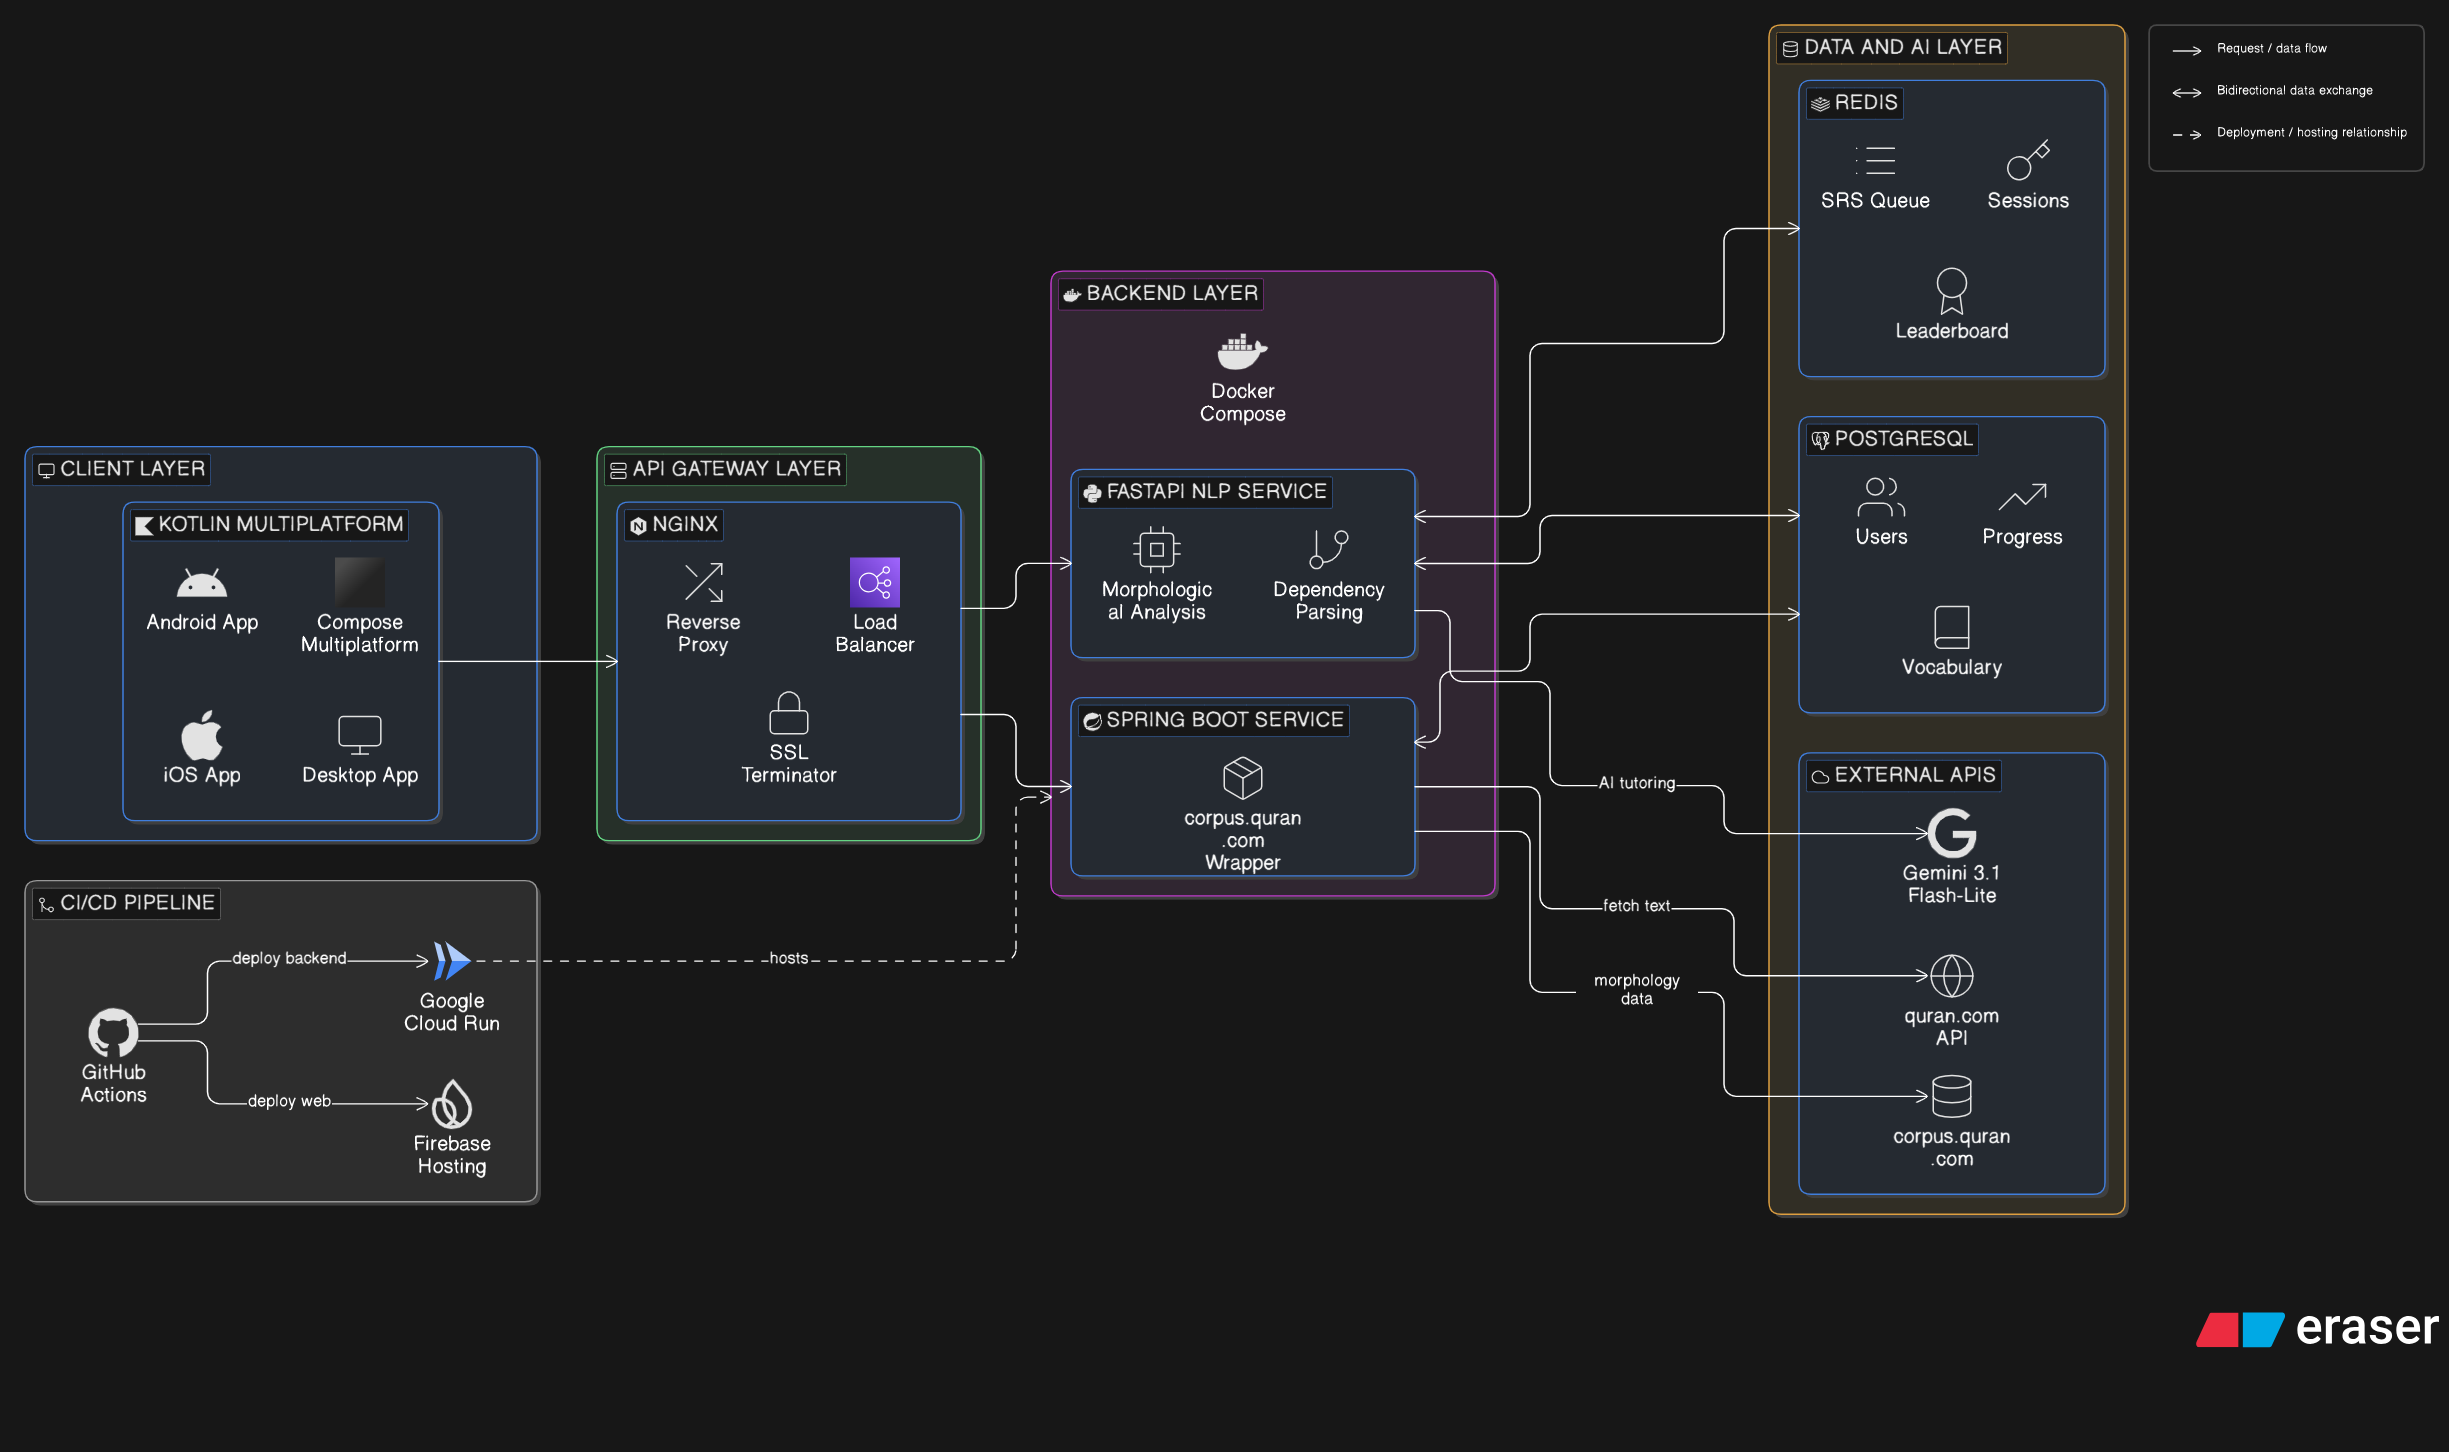
\includegraphics[width=1\linewidth]{diagrams/architecture-diagram.png}
%     \caption{High-Level System Architecture and Data Flow of the Platform}
%     \label{fig:architecture}
% \end{figure}

\begin{figure}[H]
    \centering
    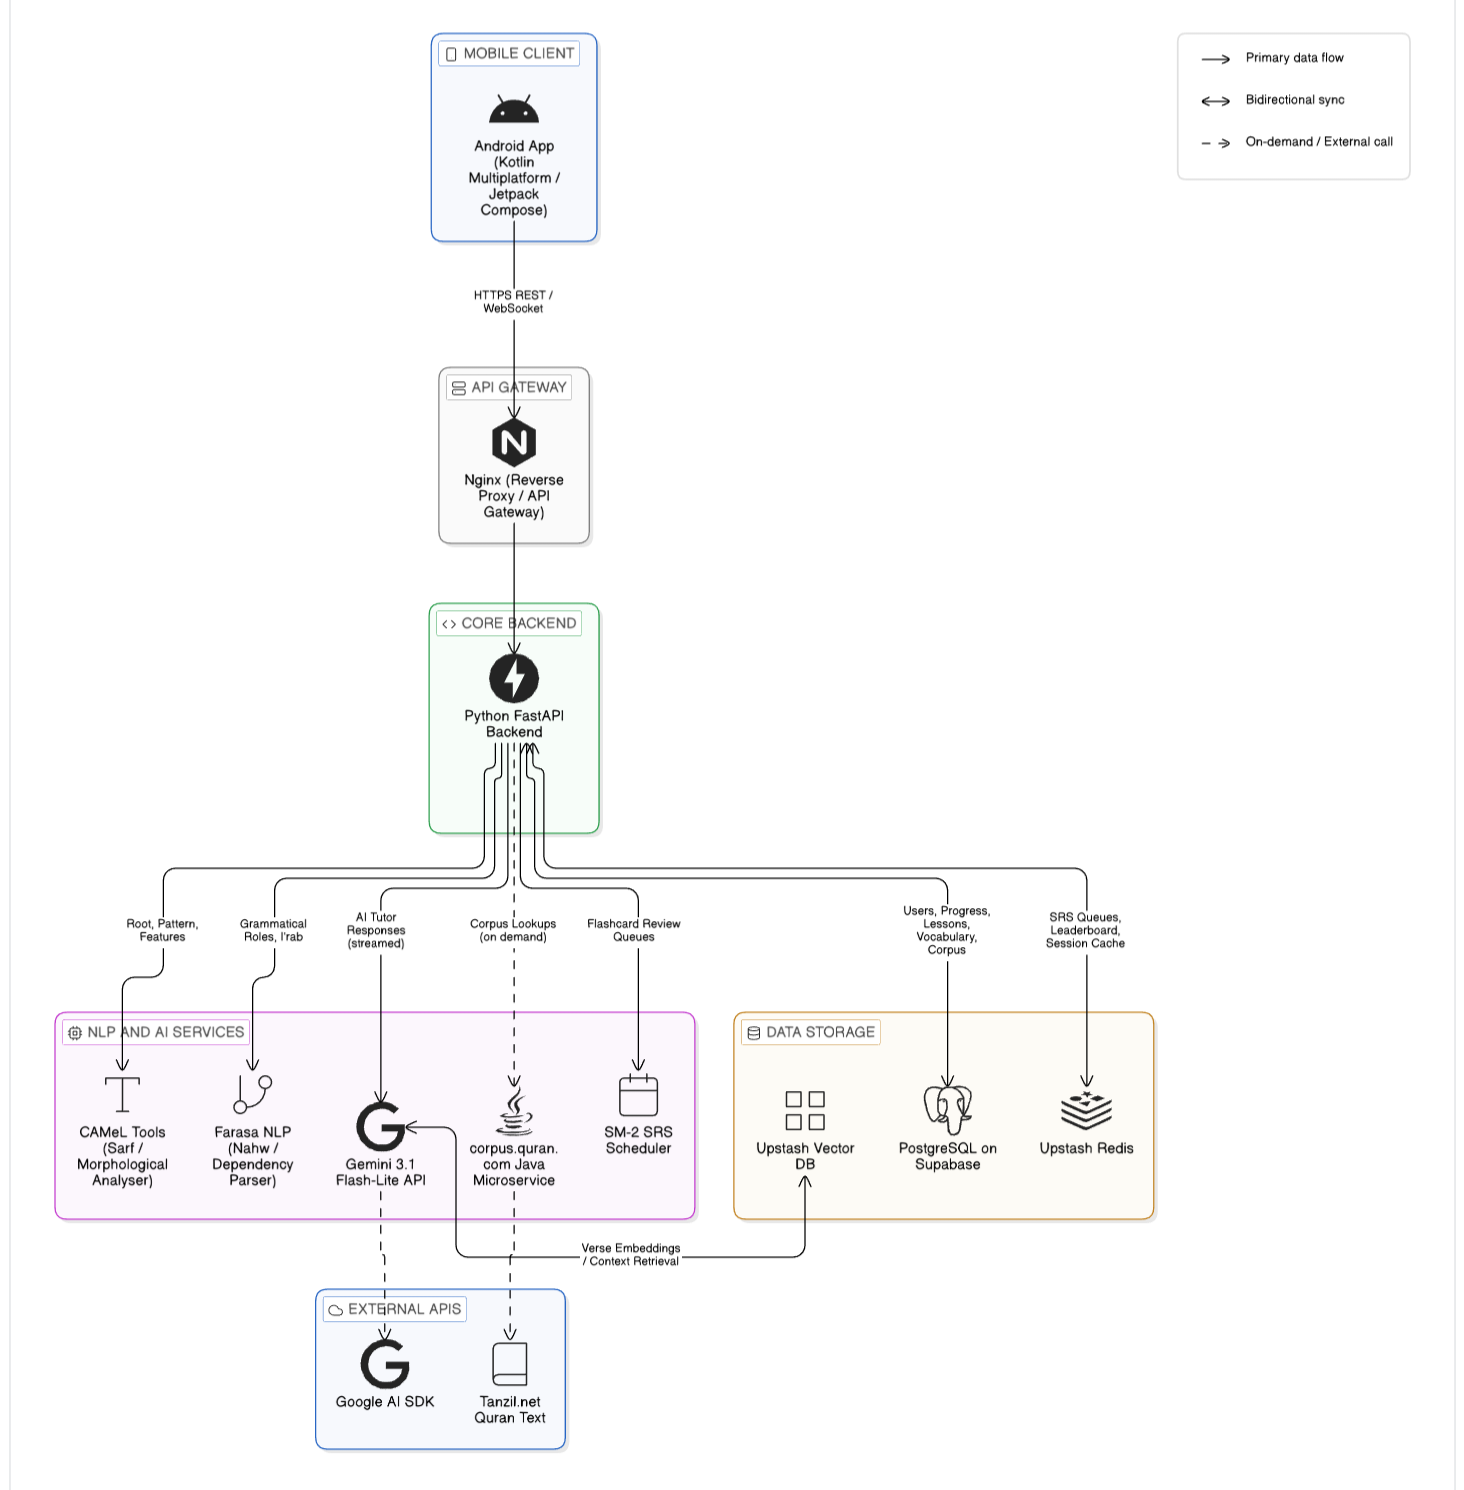
\includegraphics[width=1.1\linewidth]{diagrams/system_workflow.png}
    \caption{System Workflow}
    \label{fig:placeholder}
\end{figure}

\subsection{Sarf Engine (Morphological Analyser)}

The Sarf Engine is the morphological core of the platform, powered by CAMeL Tools running inside
the Python FastAPI backend. When a user submits any Arabic word, the engine calls the CAMeL Tools
morphological disambiguator, which analyses the word in context and returns its three-letter root
(juzr), verb pattern (bab), lemma, part of speech, and full grammatical features including tense,
voice, gender, number, and person. The module also queries the PostgreSQL corpus table, populated
from the Quranic Arabic Corpus, to return all Quranic occurrences of that root, allowing learners
to see how the same root manifests in different morphological forms across the Quran. A Word
Family Explorer sub-feature visualises the full derivative tree of a given root, enabling learners
to study related nouns, verbs, and participles together. The module covers all 32 classical verb
forms (awzan) with conjugation tables across tenses and persons, giving learners a complete
reference for Arabic verb morphology.

\subsection{Nahw Parser (Syntactic Annotator)}

The Nahw Parser uses Farasa's dependency parser, integrated into the Python FastAPI service, to
perform automated syntactic analysis of any Arabic sentence or Quranic ayah. The output is a
colour-coded, word-by-word grammatical annotation rendered on the mobile frontend: green for
fa'il (subject), blue for maf'ul bihi (object), orange for khabar (predicate), yellow for
mubtada (topic), and purple for na't (adjective modifier). Tapping any word in the annotation
view opens a detail panel showing that word's full i'rab analysis, including its grammatical
case, the reason for that case, and its syntactic dependency head. This brings the annotation
depth of the Quranic Arabic Corpus into an interactive, touch-driven interface accessible to
beginners without prior training in dependency grammar.

\subsection{AI Tutor Chatbot}

The AI Tutor is a conversational agent built on the Gemini 3.1 Flash-Lite API, configured with
a system prompt that grounds its behaviour in Classical Arabic pedagogy. The tutor is capable of
explaining any Quranic verse with a morphological and grammatical breakdown, answering grammar
questions about Sarf and Nahw in plain language, generating interactive quizzes tailored to the
learner's current level, and providing contextual explanations of individual ayaat. The tutor
maintains a conversation history within each session and adjusts the complexity of its
explanations based on the learner's assessed proficiency level stored in PostgreSQL. Chat
messages are streamed to the mobile client over WebSocket to minimise perceived latency.

\subsection{Vocabulary SRS System}

The Vocabulary SRS module implements the SM-2 spaced repetition algorithm to schedule daily
flashcard reviews from a database of Quranic vocabulary. Each flashcard contains the Arabic
word rendered in large Uthmani script, its transliteration, root, English meaning, and a
contextual verse from the Quran. After attempting recall, the learner rates the card on a
four-point scale (Again, Hard, Good, Easy), and the SM-2 algorithm recalculates the card's
ease factor and the next review interval accordingly. Review queues for each user are cached
in Upstash Redis for low-latency access. The vocabulary database is pre-populated with words
from the Quranic Arabic Corpus, grouped by frequency and root family, so that learners
encounter the most impactful vocabulary first and build root-level pattern recognition
over time.

% \begin{figure}[H]
%     \centering
%     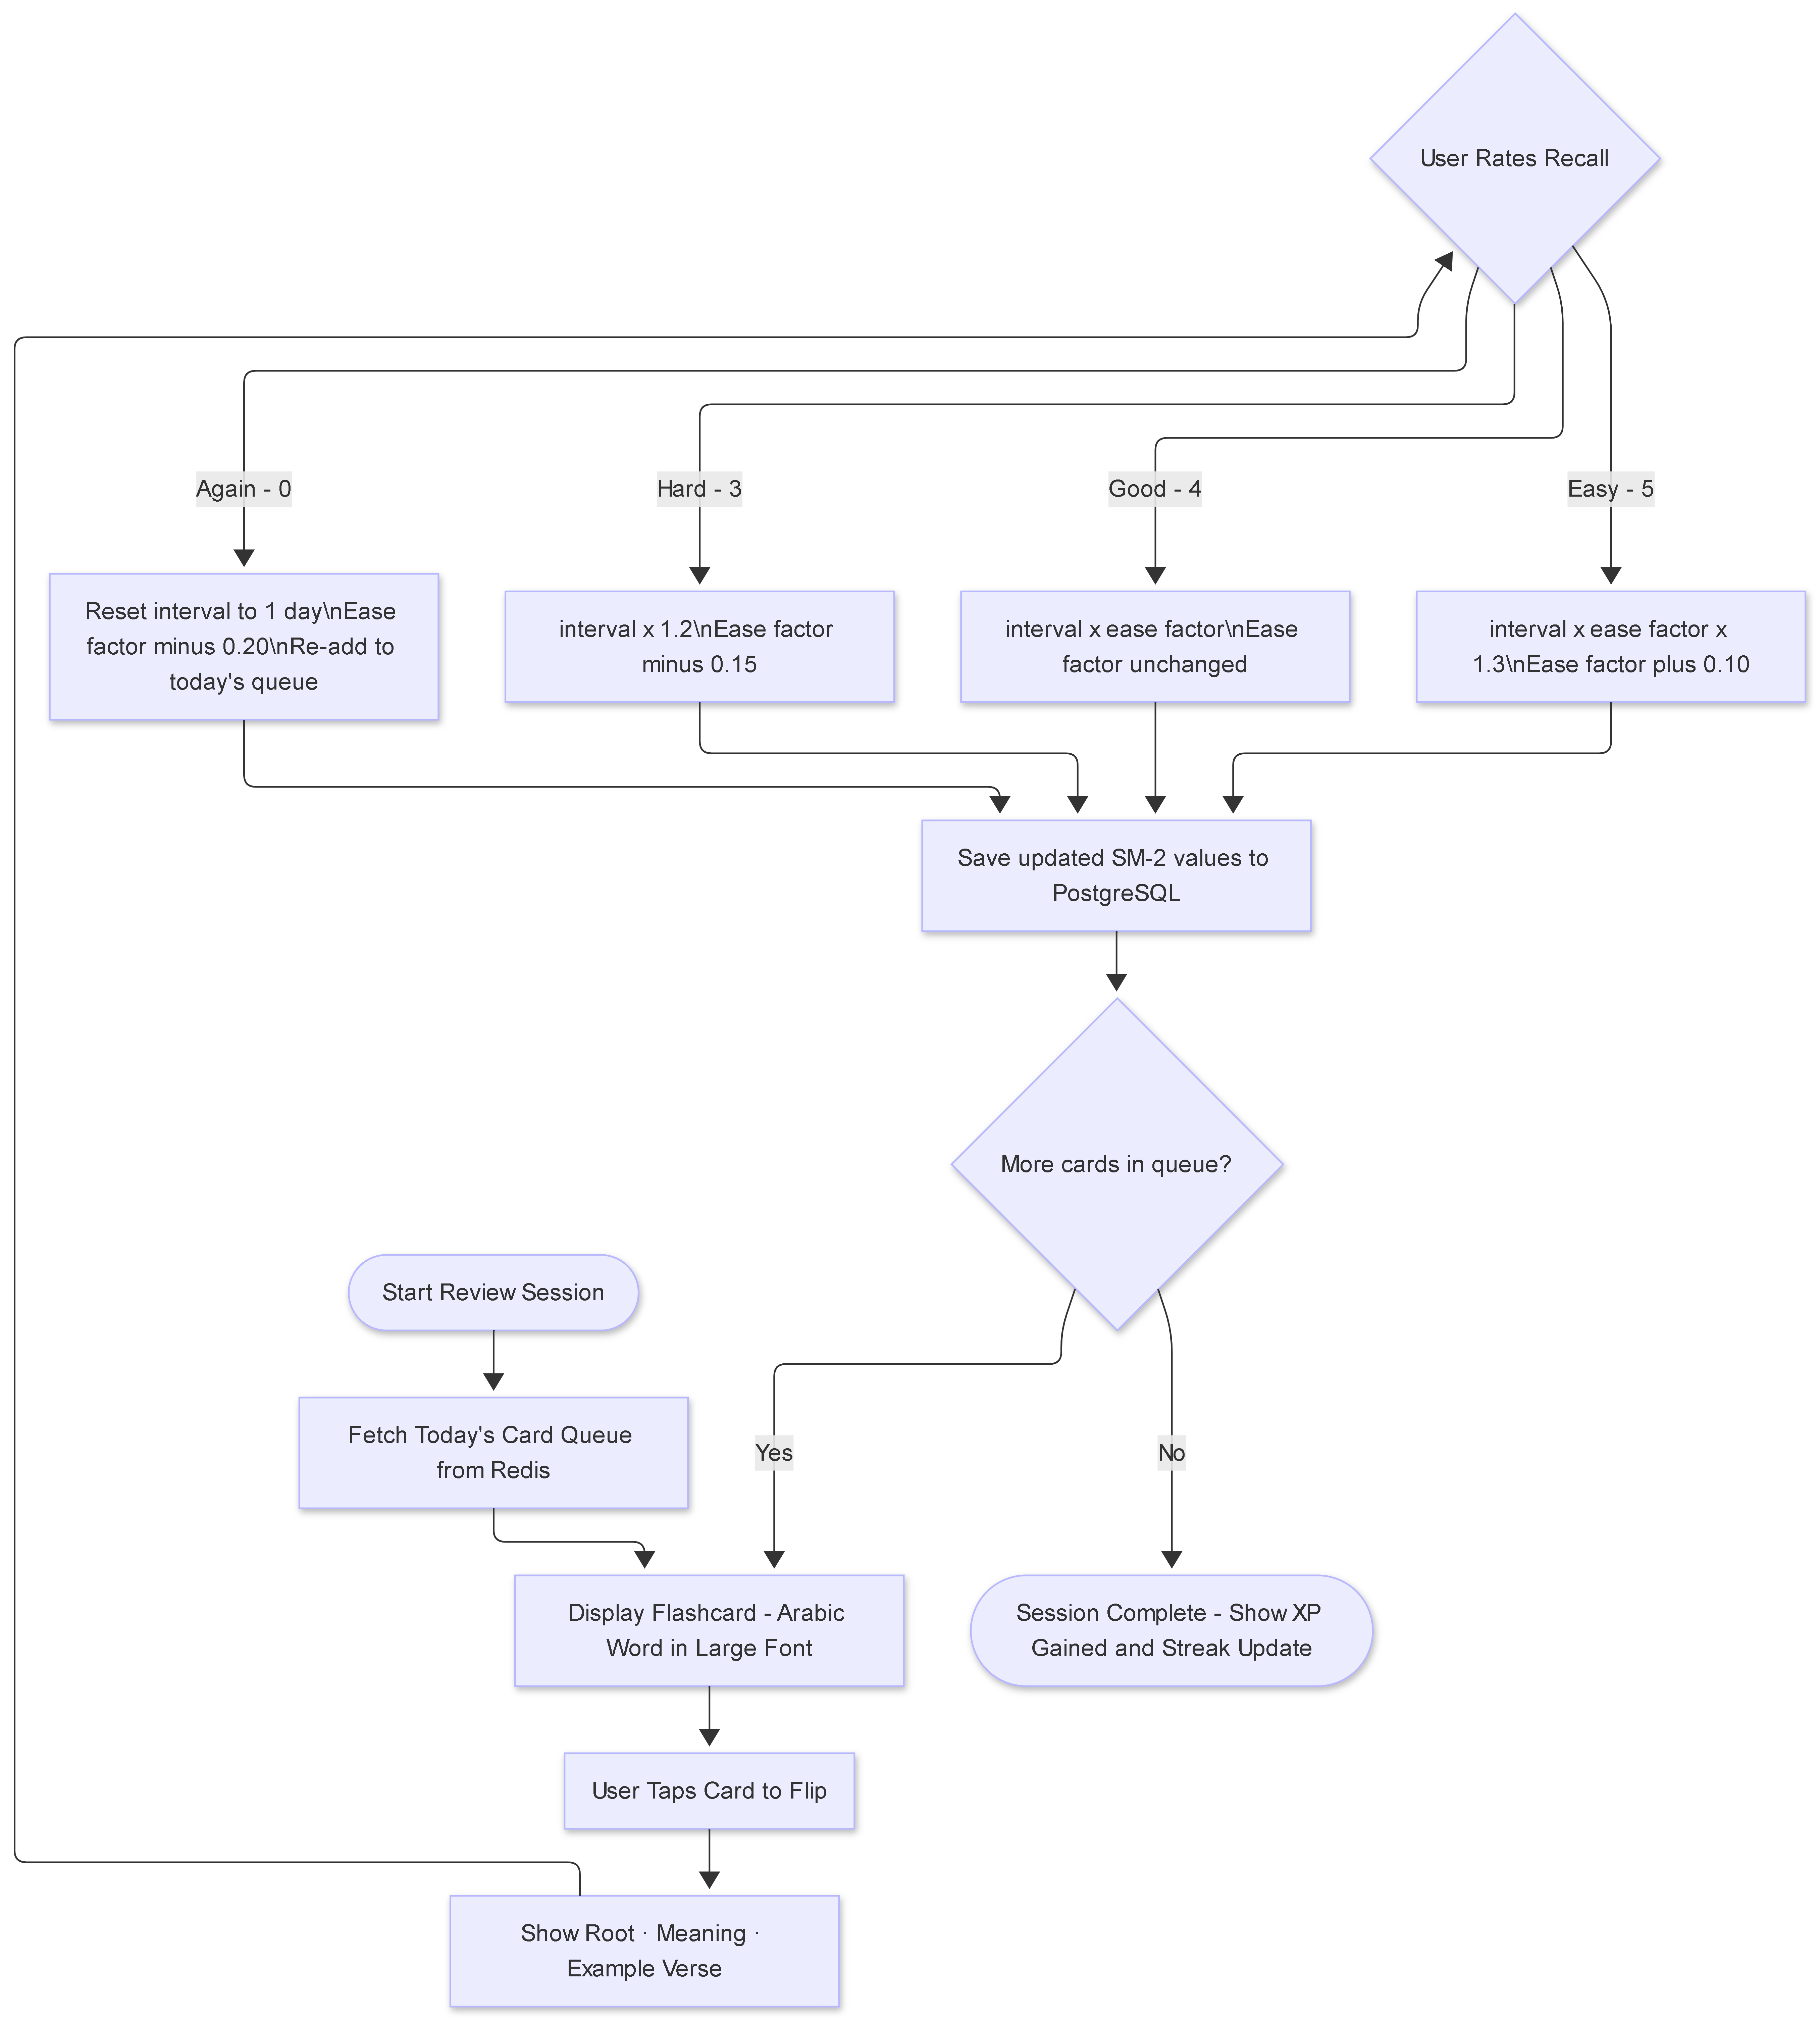
\includegraphics[width=0.75\linewidth]{diagrams/sme-flowchart.png}
%     \caption{SME: Flowchart of SME-2 Algorithm}
%     \label{fig:gantt}
% \end{figure}


\subsection{Adaptive Learning Path}

The Adaptive Learning Path module provides each user with a personalised curriculum based on
their demonstrated knowledge. On first login, the learner completes a 20-question onboarding
assessment covering vocabulary recognition, morphological pattern identification, and syntactic
role labelling. The system analyses the results and assigns a starting level across three
dimensions: vocabulary, Sarf, and Nahw. It then unlocks lessons sequentially, requiring
demonstrated competency before advancing. A weak area detection algorithm monitors per-topic
quiz performance across all sessions and automatically schedules remedial exercises in areas
where the learner's accuracy falls below a defined threshold. All progress data is stored in
PostgreSQL and rendered on the dashboard as a progress bar and topic-level heatmap.

\subsection{Quran Browser}

The Quran Browser is the primary content navigation module. It allows users to browse the
Quran by Surah and Ayah, read the Arabic text in Uthmani script with interlinear
transliteration and translation, and tap any individual word to trigger an inline morphological
popup showing its root, pattern, lemma, and grammatical features. For Quranic corpus lookups,
the backend makes a targeted call to the Java microservice that wraps the corpus.quran.com
Java library, retrieving word-level linguistic annotations on demand. The browser also
integrates with the Sarf Engine and Nahw Parser, providing one-tap access to a full syntactic
analysis of any displayed verse.

\subsection{Gamification and Engagement Layer}

The Gamification module manages the motivational infrastructure of the platform. It tracks
daily study streaks and awards streak badges at milestones of 7, 30, and 100 consecutive days.
An achievement system provides over 30 unlockable badges tied to study volume, module
completion, quiz accuracy, and vocabulary milestones. A weekly leaderboard, backed by an
Upstash Redis sorted set, ranks users by XP earned in the current seven-day window and resets
every Monday. Daily challenges present a short task each day, such as analysing a new word,
parsing a given ayah, or completing a vocabulary set, and award bonus XP on completion.

\subsection{Admin Dashboard and CMS}

The Admin Dashboard is a management interface that allows platform administrators to manage
user accounts and roles, add and edit lesson content and quiz questions, monitor aggregate
learning analytics, and push targeted notifications to user segments. It connects directly to
the Python FastAPI backend and the PostgreSQL database hosted on Supabase. The CMS component
allows content editors to update lesson text, add new vocabulary sets, and configure daily
challenges without touching application code.

% -----------------------------------------------
% Section 6: Vision Statement
% -----------------------------------------------
\section{Vision Statement}

The vision of this project is to become the world's most accessible, AI-powered gateway for
Muslims and Arabic learners to understand the Quran in its original language. Classical Arabic
grammar education has historically been confined to the classroom, the madrassa, or expensive
private tuition, making it effectively unreachable for the hundreds of millions of self-motivated
learners who lack access to qualified teachers or the financial means to pay for them. This
platform challenges that reality by making rigorous Sarf and Nahw instruction free, self-paced,
and available on any Android device, at any time, in any part of the world.

Beyond individual learners, the platform aspires to serve as a replicable model for how modern
NLP research can be brought out of the academic domain and into the hands of everyday users. The
tools that power this system, namely CAMeL Tools, Farasa, and the Quranic Arabic Corpus, have
existed in research literature for over a decade, yet no one has packaged them into a coherent
consumer product accessible to a Muslim learner in rural Pakistan or sub-Saharan Africa. This
project makes that translation concrete and deployable.

Ultimately, the goal is to enable a generation of Quran learners who do not simply read the words
of the Quran, but genuinely understand their grammatical structure, morphological roots, and
linguistic relationships, building a connection with the text that goes beyond translation and
into true comprehension.

% -----------------------------------------------
% Section 7: Scope
% -----------------------------------------------
\section{Scope}

\subsection*{In Scope}
\begin{itemize}[leftmargin=1.5em]
    \item Classical Quranic Arabic (not Modern Standard Arabic or dialects)
    \item Native Android application using Kotlin Multiplatform (Android 8.0 / API 26 and above)
    \item Python FastAPI service for CAMeL Tools and Farasa NLP processing
    \item corpus.quran.com Java library integrated as a lightweight on-demand microservice
    \item Sarf Engine: root analysis, conjugation tables, word families (32 modules total)
    \item Nahw Parser: grammatical role annotation for Quranic sentences
    \item AI Tutor chatbot using Gemini 3.1 Flash-Lite API
    \item Vocabulary SRS system with SM-2 algorithm
    \item Adaptive learning path with onboarding assessment
    \item Gamification: daily challenges, streaks, badges, leaderboards
    \item User authentication and progress tracking
\end{itemize}

\subsection*{Out of Scope}
\begin{itemize}[leftmargin=1.5em]
    \item Tajweed (Quranic recitation rules) and audio-based pronunciation correction
    \item Hifz (memorisation) features, which are already addressed by Tarteel AI
    \item Modern Standard Arabic or colloquial Arabic dialects
    \item Desktop and web platform support (mobile is the current focus)
    \item Mobile offline mode (Phase 1 requires an internet connection)
    \item Paid subscription or monetisation system (the platform will be free)
\end{itemize}

% -----------------------------------------------
% Section 8: Methodology
% -----------------------------------------------
\section{Methodology}

The system will be developed using an Agile methodology divided into nine one-month sprints,
each delivering a testable and reviewable increment. The development follows a modular
architecture that allows frontend, backend, and AI/NLP components to be built in parallel.

\textbf{Phase 1 -- Requirements \& Design:} Stakeholder analysis,
system requirements specification, database schema design, and Quran data pipeline planning.
The corpus.quran.com morphological dataset will be ingested into PostgreSQL on Supabase as
the primary linguistic reference. Docker configurations will be set up for the Python backend
and the Java microservice.

\textbf{Phase 2 -- Core Backend \& Vocabulary SRS:} User
authentication (JWT + bcrypt), user profile management, PostgreSQL schema deployment, and
full implementation of the Flashcard SRS module with SM-2 scheduling. Upstash Redis is
configured for SRS queue and session caching. The corpus.quran.com Java microservice is
built, containerised, and tested against the corpus.

\textbf{Phase 3 -- Sarf Engine:} Integration of CAMeL Tools
morphological analyser via the Python FastAPI service. Development of the Root Analyser,
Verb Conjugation Trainer, Word Family Explorer, and Morphological Pattern Library modules.
Unit testing against the corpus.quran.com gold standard.

\textbf{Phase 4 -- Nahw Parser \& AI Tutor:} Integration of
Farasa NLP dependency parser into the Python backend. Development of the Nahw Parser UI
with colour-coded grammatical role annotation. Gemini 3.1 Flash-Lite API integration for
the AI Tutor with a Classical Arabic pedagogy system prompt and WebSocket streaming for
real-time chat responses.

\textbf{Phase 5 -- Personalisation \& Mobile App:} Adaptive
learning path engine, 20-question onboarding assessment, weak area detection algorithm,
gamification layer (streaks, badges, leaderboard), and native Android application development
using Kotlin Multiplatform with Jetpack Compose.

\textbf{Phase 6 -- Quran Browser:} Development
of the Quran Browser with Uthmani script rendering, interlinear translation, and word-tap
morphological popups.

\textbf{Phase 7 -- Integration \& System Testing:} End-to-end
integration testing across all services, Nginx gateway and reverse proxy validation,
morphological accuracy benchmarking against corpus.quran.com, and performance and load
testing with bug fixing and stability improvements.

\textbf{Phase 8 -- User Study \& Evaluation:} User study with 30
participants using pre/post learning assessments, AI Tutor quality evaluation by an Arabic
language expert, SRS retention analysis, UI/UX feedback collection and iteration, and
GitHub Actions CI/CD pipeline finalisation.

\textbf{Phase 9 -- Documentation \& Final Submission:} FYP final
report writing, API documentation via OpenAPI/Swagger, codebase cleanup and refactoring,
final presentation preparation, and project submission and viva.
% -----------------------------------------------
% Section 9: Tools and Technologies
% -----------------------------------------------
\section{Tools and Technologies}

\begin{itemize}[leftmargin=1.5em]

    \item \textbf{Mobile Frontend:}
    Kotlin Multiplatform (Android 8.0 / API 26+), Jetpack Compose, Material Design 3.

    \item \textbf{Backend (NLP and API):}
    Python, FastAPI, CAMeL Tools (Sarf morphological analyser), Farasa (Nahw dependency parser),
    Docker, Google Cloud Run / Oracle Cloud Free Tier, Nginx.

    \item \textbf{Corpus Microservice:}
    corpus.quran.com Java library, lightweight Java process, Docker.

    \item \textbf{Database:}
    PostgreSQL on Supabase.

    \item \textbf{Caching and Queue:}
    Upstash Redis (SRS queues, leaderboard sorted sets, session caching),
    Upstash Vector (sentence embeddings for AI Tutor context retrieval).

    \item \textbf{AI Model:}
    Gemini 3.1 Flash-Lite API (Google DeepMind), Google AI SDK.

    \item \textbf{Authentication:}
    JWT (JSON Web Tokens), bcrypt.

    \item \textbf{API Gateway and Reverse Proxy:}
    Nginx (SSL termination, request routing, rate limiting).

    \item \textbf{Version Control:}
    Git, GitHub (feature branching, pull requests, code review).

    \item \textbf{CI/CD and DevOps:}
    GitHub Actions (automated testing, Docker image builds, cloud deployment), Docker, Docker Compose.

    \item \textbf{Development Tools:}
    NeoVim, Android Studio, VS Code, Postman (API testing), pgAdmin (database management).

    \item \textbf{Project Management:}
    GitHub Projects (sprint planning, issue tracking, milestone management).

    \item \textbf{Deployment Platform:}
    Oracle Cloud, Google Cloud.

\end{itemize}
% -----------------------------------------------
% Section 10: Applications
% -----------------------------------------------
\section{Applications of this Project}

This platform has a wide range of educational, social, and technological applications:

\begin{itemize}[leftmargin=1.5em]
    \item \textbf{Quranic comprehension for self-learners:} Any Muslim worldwide can use this
    platform to progress from basic word recognition to a full grammatical understanding of
    Quranic Arabic, without needing a human teacher.

    \item \textbf{University Arabic curricula:} The platform can serve as a digital learning management
    tool for Arabic language departments in universities across Pakistan and other Muslim-majority
    countries.

    \item \textbf{Madrassa and Islamic school supplement:} It provides an interactive, self-paced
    supplement to traditional Nahw and Sarf textbooks such as Al-Ajurrumiyyah and Tayseer al-Sarf.

    \item \textbf{Arabic NLP research:} Integrating CAMeL Tools and Farasa within a real-world
    pedagogical interface creates a practical evaluation testbed for Arabic NLP tools in
    educational settings.

    \item \textbf{Convert and revert communities:} New Muslims and those returning to practice who
    want to connect with the Quran linguistically but have no prior Arabic background.

    \item \textbf{Pakistani Muslim community:} With over 230 million Muslims, Pakistan is home to the
    world's largest non-native Arabic-speaking Muslim population, making it the primary target
    user base for the platform's initial deployment.
\end{itemize}

% -----------------------------------------------
% Section 11: WBS and Gantt Chart
% -----------------------------------------------
\section{WBS and Gantt Chart}



\begin{figure}[H]
    \centering
    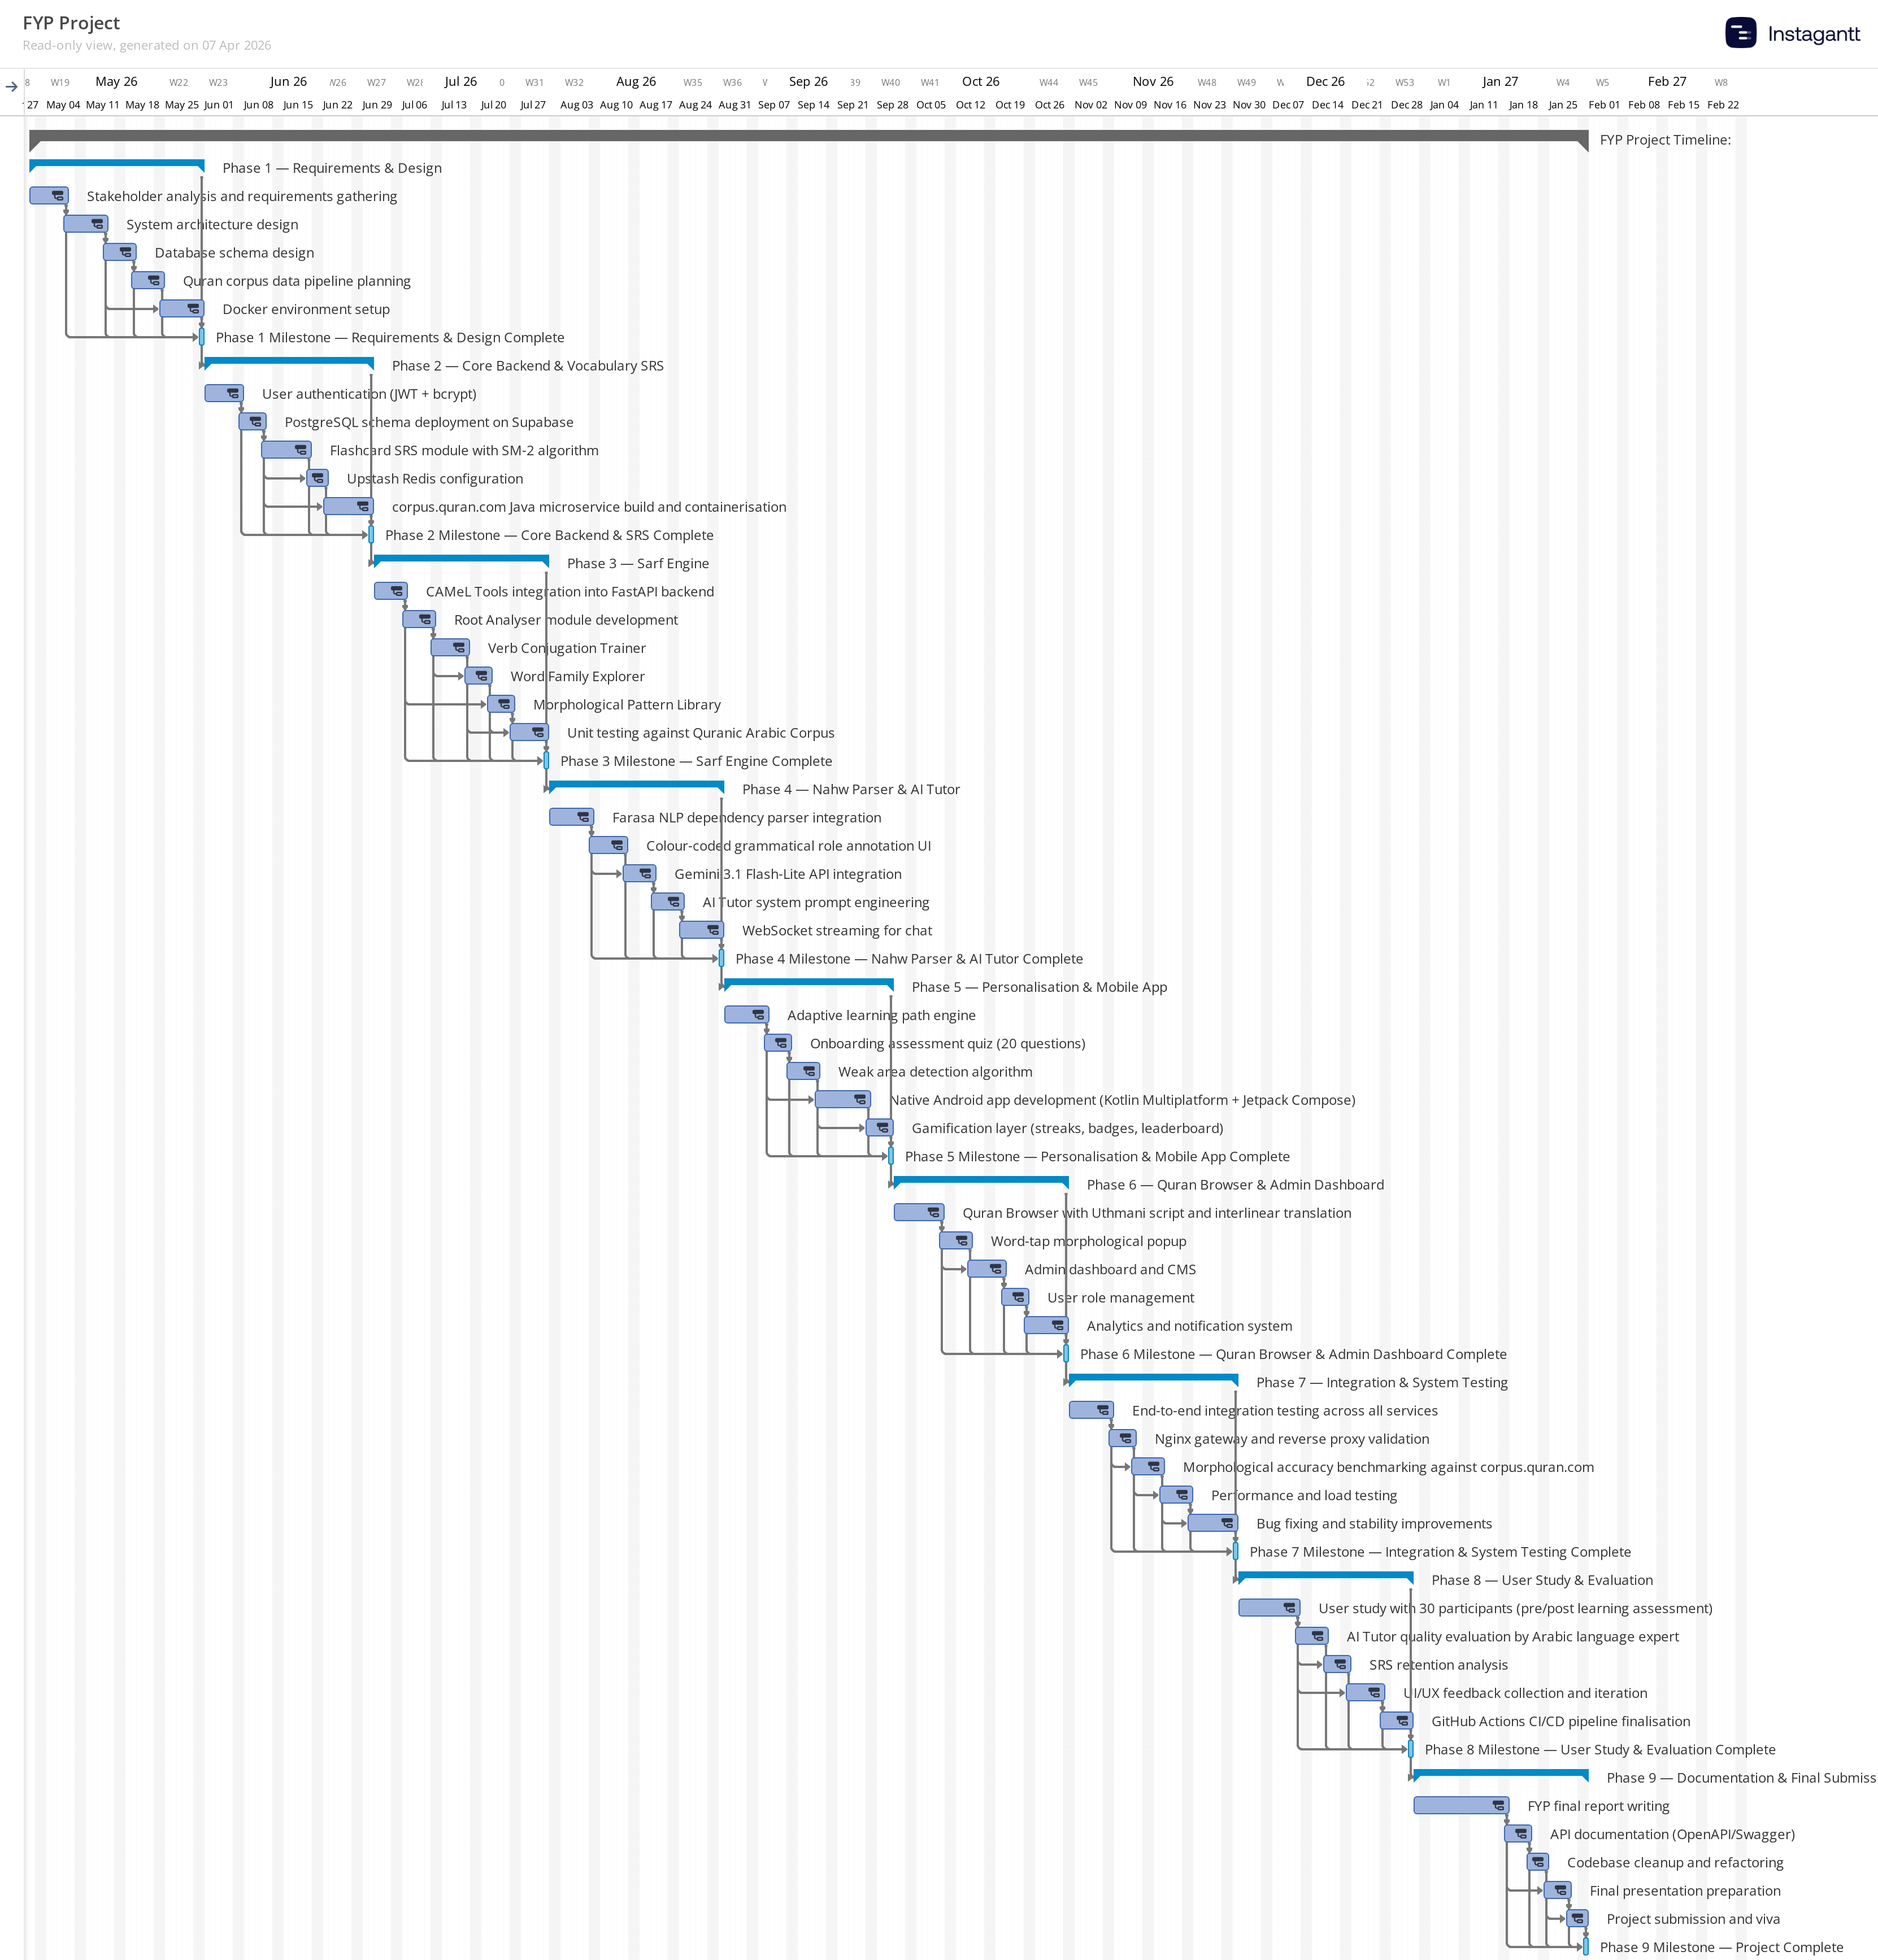
\includegraphics[width=1.0\linewidth]{diagrams/ghanttchart_instaghanntt.png}
    \caption{Gantt Chart: Nine-Month Development Timeline}
    \label{fig:gantt}
\end{figure}

% -----------------------------------------------
% Section 12: Mockups
% -----------------------------------------------
\section{Mockups}

\begin{figure}[H]
    \centering
    \begin{minipage}[t]{0.48\textwidth}
        \centering
        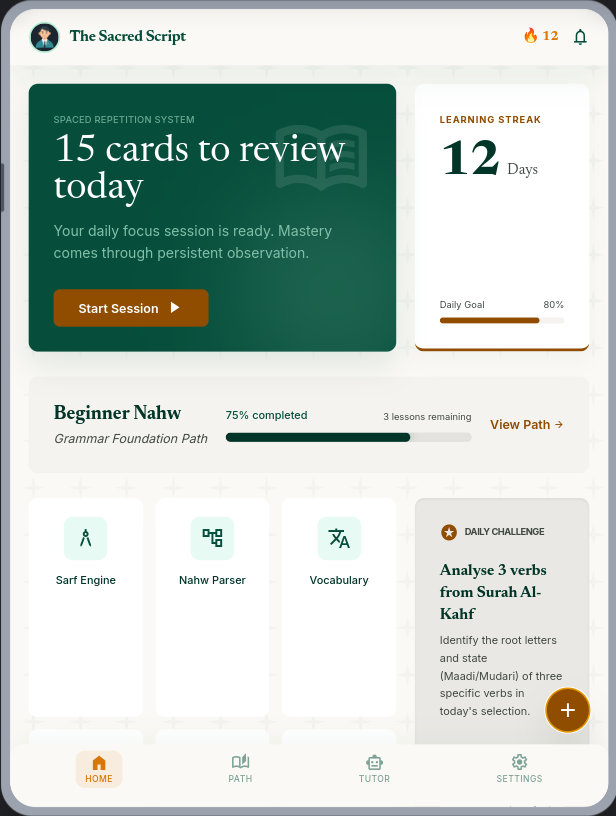
\includegraphics[width=0.9\linewidth]{mockups/dashboard.png}
        \caption{Dashboard Mockup UI}
        \label{fig:dashboard}
    \end{minipage}
    \hfill
    \begin{minipage}[t]{0.48\textwidth}
        \centering
        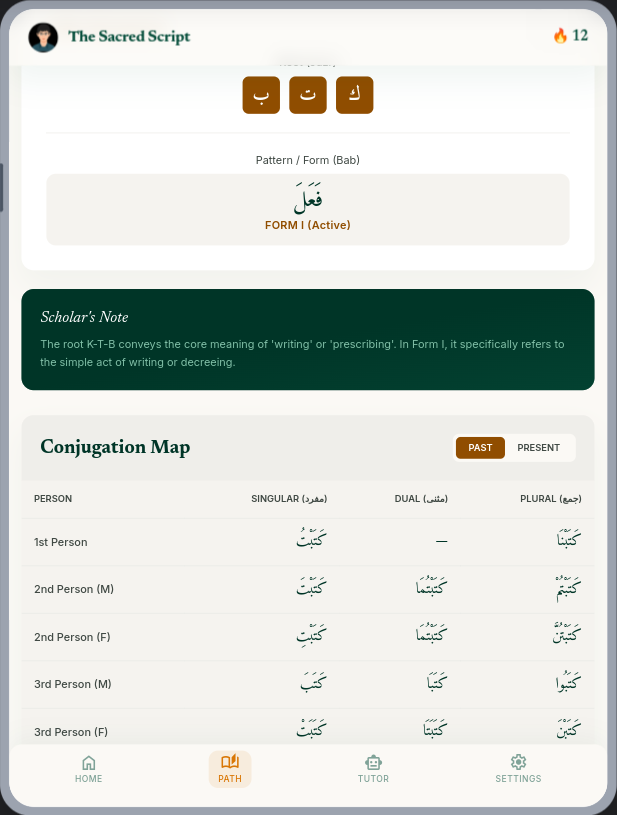
\includegraphics[width=0.9\linewidth]{mockups/sarf_engine.png}
        \caption{Sarf Engine Mockup UI}
        \label{fig:sarf}
    \end{minipage}

    \vspace{1em}

    \begin{minipage}[t]{0.48\textwidth}
        \centering
        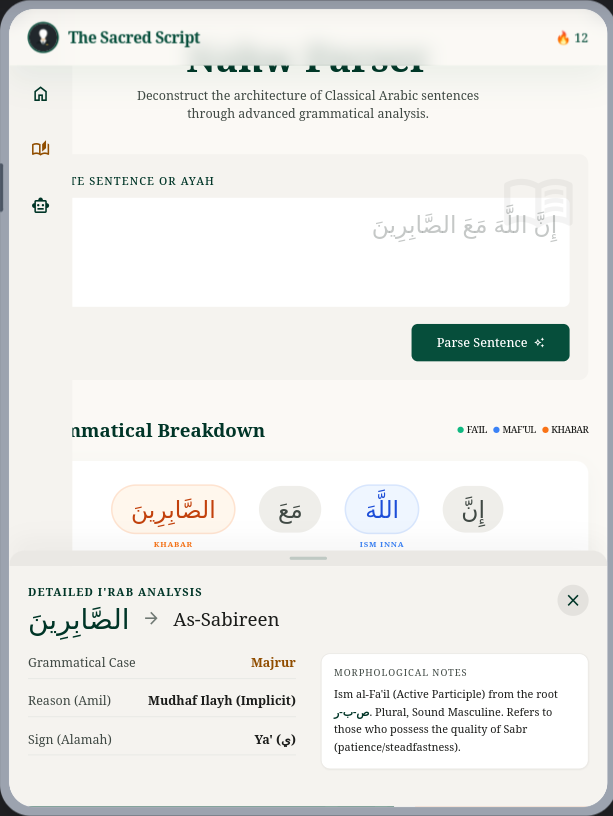
\includegraphics[width=0.9\linewidth]{mockups/nahw_parser.png}
        \caption{Nahw Parser Mockup UI}
        \label{fig:nahw}
    \end{minipage}
    \hfill
    \begin{minipage}[t]{0.48\textwidth}
        \centering
        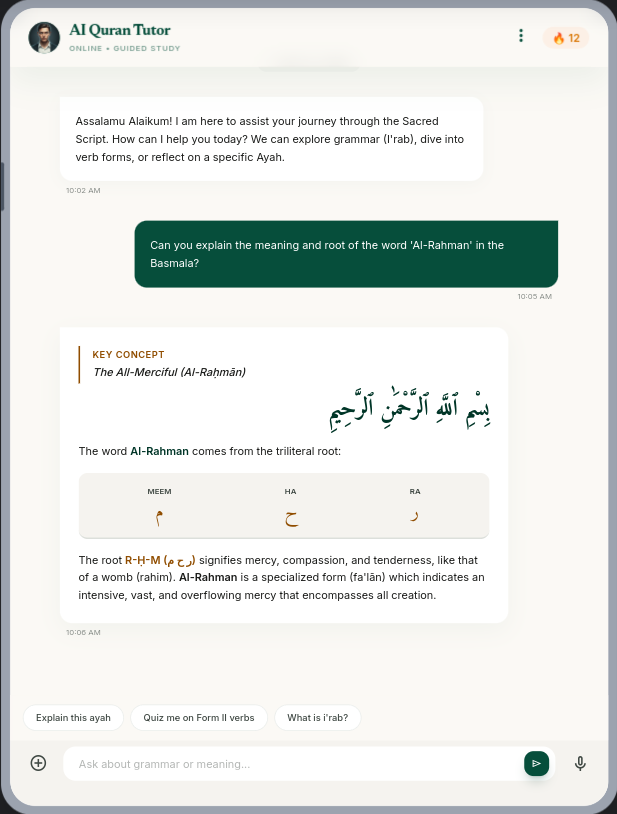
\includegraphics[width=0.9\linewidth]{mockups/ai_tutor.png}
        \caption{AI Tutor Mockup UI}
        \label{fig:aitutor}
    \end{minipage}
\end{figure}

\begin{figure}[H]
    \centering
    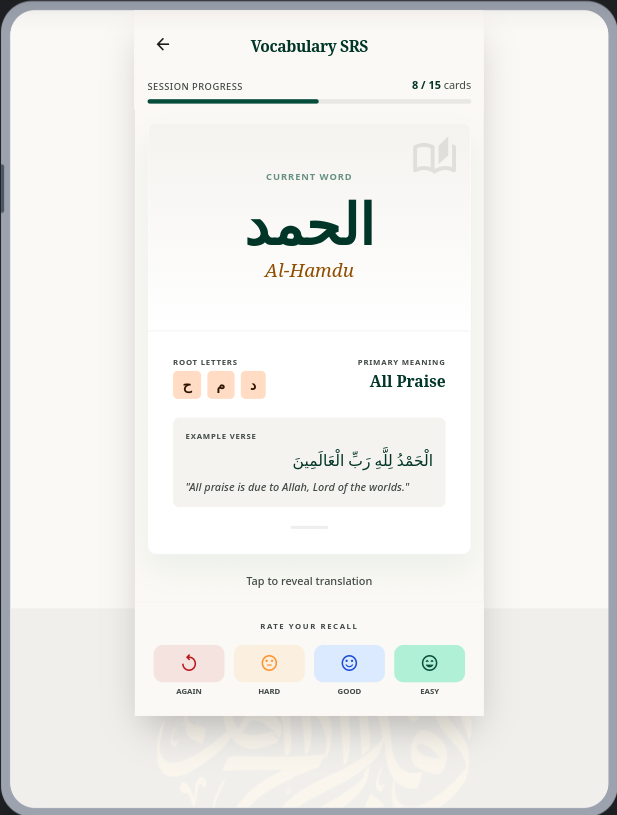
\includegraphics[width=0.5\linewidth]{mockups/flashcard.png}
    \caption{Flashcard Screen Mockup UI}
    \label{fig:flashcard}
\end{figure}

% -----------------------------------------------
% References
% -----------------------------------------------
\newpage
\begin{thebibliography}{9}


\bibitem{dukes2010}
Kais Dukes and Nizar Habash.
\textit{Morphological annotation of {Q}uranic {A}rabic.}
Proceedings of the Language Resources and Evaluation Conference (LREC),
pages 2530--2536, 2010.
Available: \url{http://corpus.quran.com}.

\bibitem{habash2010}
Nizar Y. Habash.
\textit{Introduction to Arabic Natural Language Processing.}
Synthesis Lectures on Human Language Technologies, vol.~10.
Morgan \& Claypool, 2010.
ISBN 978-1-59829-795-9.

\bibitem{atwell2010}
Eric Atwell, Nizar Habash, William Magdy, Abdallah Sharaf, and Kais Dukes.
\textit{Understanding the {Q}ur'an: A new grand challenge for computer science
and artificial intelligence.}
In Proceedings of the ACS/IEEE International Conference on Computer Systems
and Applications (AICCSA), 2010.

\bibitem{bashir2022}
Muhammad Huzaifa Bashir, Aqil M. Azmi, Haq Nawaz, Wajdi Zaghouani, Mona Diab,
Ala Al-Fuqaha, and Junaid Qadir.
\textit{Arabic natural language processing for {Q}ur'anic research: a systematic review.}
Artificial Intelligence Review, vol.~56, no.~7, pages 6801--6854, December 2022.
\url{https://doi.org/10.1007/s10462-022-10313-2}.

\bibitem{obeid2020}
Ossama Obeid, Nasser Zalmout, Salam Khalifa, Dima Taji, Mai Oudah, Bashar Alhafni,
Go Inoue, Fadhl Eryani, Alexander Erdmann, and Nizar Habash.
\textit{{CAMeL} tools: An open source python toolkit for Arabic natural language processing.}
In Proceedings of the 12th Language Resources and Evaluation Conference,
pages 7022--7032. European Language Resources Association, 2020.
New York University Abu Dhabi.

\bibitem{abdelali2016}
Ahmed Abdelali, Kareem Darwish, Nadir Durrani, and Hamdy Mubarak.
\textit{Farasa: A fast and furious segmenter for Arabic.}
In Proceedings of the 2016 Conference of the North American Chapter of the
Association for Computational Linguistics: Demonstrations, pages 11--16.
Association for Computational Linguistics, 2016.
Qatar Computing Research Institute (QCRI).

\bibitem{ebbinghaus1885}
Hermann Ebbinghaus.
\textit{Memory: A Contribution to Experimental Psychology.}
Columbia University Press, 1885.
Extended by Wozniak, P.A. SM-2 spaced repetition algorithm, SuperMemo, 1990.

% ── NEW REFERENCES ──────────────────────────────────────────────────────────

\bibitem{farghaly2009}
Ali Farghaly and Khaled Shaalan.
\textit{Arabic natural language processing: Challenges and solutions.}
ACM Transactions on Asian Language Information Processing,
vol.~8, no.~4, article~14, 2009.
\url{https://doi.org/10.1145/1644879.1644881}.

\bibitem{pasha2014}
Arfath Pasha, Mohamed Al-Badrashiny, Mona Diab, Ahmed El Kholy,
Ramy Eskander, Nizar Habash, Manoj Pooleery, Owen Rambow, and Ryan Roth.
\textit{{MADAMIRA}: A fast, comprehensive tool for morphological analysis
and disambiguation of Arabic.}
In Proceedings of the Ninth International Conference on Language Resources
and Evaluation (LREC), pages 1094--1101.
European Language Resources Association, 2014.

\bibitem{taji2017}
Dima Taji, Nasser Zalmout, and Nizar Habash.
\textit{Universal dependencies for Arabic.}
In Proceedings of the Third Arabic Natural Language Processing Workshop,
pages 166--176. Association for Computational Linguistics, 2017.
\url{https://doi.org/10.18653/v1/W17-1320}.

\bibitem{settles2016}
Burr Settles and Brendan Meeder.
\textit{A trainable spaced repetition model for language learning.}
In Proceedings of the 54th Annual Meeting of the Association for
Computational Linguistics (ACL), volume~1 (Long Papers),
pages 1848--1858. Association for Computational Linguistics, 2016.
\url{https://doi.org/10.18653/v1/P16-1174}.

\bibitem{seibert2020}
Aroline E. Seibert Hanson and Charles M. Brown.
\textit{Enhancing {L2} learning through a mobile assisted spaced-repetition
tool: an effective but bitter pill?}
Computer Assisted Language Learning, vol.~33, no.~1--2,
pages 133--155, 2020.
\url{https://doi.org/10.1080/09588221.2018.1552975}.

\bibitem{kim2022}
Soo Kim and Stuart Webb.
\textit{The effects of spaced practice on second language learning:
A meta-analysis.}
Language Learning, vol.~72, no.~1, pages 269--319, 2022.
\url{https://doi.org/10.1111/lang.12479}.

\bibitem{zhang2024}
Zhihui Zhang and Xiaomeng Huang.
\textit{The impact of chatbots based on large language models on second
language vocabulary acquisition.}
Heliyon, vol.~10, no.~3, article~e25370, 2024.
\url{https://doi.org/10.1016/j.heliyon.2024.e25370}.

\bibitem{deterding2011}
Sebastian Deterding, Dan Dixon, Rilla Khaled, and Lennart Nacke.
\textit{From game design elements to gamefulness: Defining ``gamification.''}
In Proceedings of the 15th International Academic MindTrek Conference,
pages 9--15. ACM, 2011.
\url{https://doi.org/10.1145/2181037.2181040}.

\bibitem{hamari2014}
Juho Hamari, Jonna Koivisto, and Harri Sarsa.
\textit{Does gamification work? --- A literature review of empirical studies
on gamification.}
In Proceedings of the 47th Hawaii International Conference on System Sciences
(HICSS), pages 3025--3034. IEEE, 2014.
\url{https://doi.org/10.1109/HICSS.2014.377}.

\bibitem{furqan_sarf2026}
Furqan Apps.
\textit{Sarf ({$\Sigma$\!\!\!\raisebox{-0.2ex}{$\varsigma$}} -- Arabic Verb Conjugator) [Mobile application].}
Google Play Store, 2026.
Available: \url{https://play.google.com/store/apps/details?id=app.furqan.sarf}

\bibitem{furqan_quran2026}
Furqan Apps.
\textit{Quran [Mobile application].}
Google Play Store, 2026.
Available: \url{https://play.google.com/store/apps/details?id=app.furqan.irab}

\bibitem{tarteel2024}
Tarteel Inc.
\textit{Tarteel: AI Quran Memorization [Mobile application].}
Google Play Store, 2024.
Available: \url{https://play.google.com/store/apps/details?id=com.mmmoussa.iqra}

\end{thebibliography}

\end{document}